
\documentclass[12pt]{article}
\usepackage{graphicx}
\usepackage{amsmath}
\usepackage{listings}
\usepackage{color}
\usepackage{float}

\definecolor{dkgreen}{rgb}{0,0.6,0}
\definecolor{dkblue}{rgb}{0,0.0,0.6}
\definecolor{dkred}{rgb}{0.9,0.0,0.1}

\begin{document}

\lstset{language=Fortran,tabsize=4,numbers=left,numberstyle=\tiny,basicstyle=\ttfamily\small\color{dkblue},stringstyle=\ttfamily\color{blue},keywordstyle=\rmfamily\color{dkred}\bfseries\emph,backgroundcolor=\color{white},commentstyle=\color{dkgreen}}


\title{Final}
\author{Paul Fischer \\
Department of Physics\\
California State University Long Beach}
\date{May 15, 2020}

\maketitle

\begin{abstract}

In problem 1, we consider the Poisson equation for an electric potential for a spherically symmetric charge distribution.  For four given charge distributions, we plot the electric potential and electric field as a function of the radius from the center of the charge distribution and calculate the total charge.

In problem 2, we consider a table of experimental data for the reflection coefficient of a wavefunction with a distribution of incoming energies scattering off of a potential barrier.  We plot a potential barrier that has been fitted to the given data.

\end{abstract}

\section{Introduction}

Poisson's equation is a generalization of Laplace's equation, which appear in many different areas of physics.  Often Poisson's equation is solved through the method of Green's functions, but doing this analytically becomes increasingly more difficult as the charge distributions become more complex or nonlinear.  For example, this problem arises in fluid dynamics via the Navier-Stokes equations, one of the famously unsolved problems in mathematics \cite{poisson}.  This urges the power that computational physics holds, this mathematical difficulty does not prevent us from being able to numerically approximate and therefore model the interesting physics within these kinds of systems, as we do for a group of spherically symmetric charge distributions in Problem 1.

Reflection coefficients have been used to describe physical systems (like in optics) for a long time.  The wave mechanics of modern physics allows us to model particles as waves with real and imaginary parts that interacts with potential barriers, scattering with some reflection and transmission probabilities.  The understanding of the ability for a particle to tunnel through a classically impossible potential barrier marked a new era in physics, and a new era in which computational physics could greatly increase the efficiency of research \cite{reflection}.  In problem 2, we exercise this power to reconstruct a potential barrier given only data containing the reflection probability of the wave after being scattered with some distribution of incoming energies.  

This final will be organized as follows: section {\tt Problem 1} will describe the code used to solve Problem 1, section {\tt Problem 1: Figures} will contain the plots made to solve Problem 1, section {\tt Problem 2} will describe the code and the output/graphs used to solve Problem 2, and then section {\tt Summary and conclusions} will summarize and reflect upon the colutions to the problems.

\section{Problem 1}

In Problem 1, let us consider the electric potential $\Phi$ of a charge distribution $\rho(\textbf{r})$ that is determined by the Poisson equation \[\nabla^2\Phi(\textbf{r})=-4\pi\rho(\textbf{r}),\] which, for a spherically symmetric $\rho$, simplifies to \[\frac{1}{r^2}\frac{d}{dr}\left(r^2\frac{d\Phi(r)}{dr}\right)=-4\pi\rho(r).\]  We write a {\tt Fortran 90} code to plot $\Phi(r)$, the electric field $E(r)$, and the total charge $Q$ for the following four charge distributions:

\begin{enumerate}
    \begin{enumerate}
        \item $\rho(r)=\frac{1}{8\pi}e^{-r}$
        \item $\rho(r)=\frac{1}{24\pi}re^{-r}$
        \item $\rho(r)=\frac{1}{2\pi}\sin(r)e^{-r}$
        \item $\rho(r)=\frac{1}{8\pi}\cos(r)e^{-r}$
    \end{enumerate}
\end{enumerate}

We will make the substitution $\Phi=\frac{\phi}{r}$ to simplify the differential equation in the Runge-Kutta method numerical approximation: \[\frac{d^2\phi(r)}{dr^2}=-4\pi r\rho(r).\]  This substitution will yield the following plots: $\phi(r)$, $\Phi(r)=\frac{\phi(r)}{r}$, and $E(r)=-\frac{d\Phi(r)}{dr}=\frac{\phi(r)-r\frac{d\phi(r)}{dr}}{r^2}$.

The Makefile in Listing \ref{makefile} provides the instructions for the terminal on how to compile the code.  The {\tt *.f90} files have to be linked together as {\tt *.o} files in the right order, since some of them use subroutines or modules contained in the other ones.  This order is entered from left to right in {\tt objs1}.  Once the object files are linked, they are turned into an executable {\tt pot} such that the code can be run by typing {\tt ./pot} into the terminal in the directory {\tt $\sim$/src}.  The {\tt gfortran} compiler is used as well as flags for optimization. The library {\tt -framework Accelerate} which contains the linear algebra package {\tt LAPACK} is also include in the compilation instructions.  The non-{\tt *.f90} files can be removed by typing {\tt make clean} into the terminal.

\begin{lstlisting}[frame=single,caption={{\tt Makefile}},label=makefile]

objs1 = numtype.o setup.o d01b.o cheby.o rk4step.o elpot.o 

prog1 = pot

f90 = gfortran

f90flags = -O3 -funroll-loops -ftree-vectorize -fexternal-blas

libs = -framework Accelerate

ldflags = $(libs)

all: $(prog1)

$(prog1): $(objs1)
	$(f90) $(ldflags) -o $@ $(objs1)

clean: 
	rm -f $(prog1) *.{o,mod} fort.*

.suffixes: $(suffixes) .f90

%.o: %.f90
	$(f90) $(f90flags) -c $<

\end{lstlisting}

The file {\tt numtype.f90} in Listing \ref{numtype} contains the module {\tt numtype}, which we use to define the precision {\tt dp} of our floating point data types.  We also define the constant {\tt pi}$\equiv\pi$, the complex number {\tt iic}$\equiv i$, and a parameter for very small floating point real data types {\tt tiny}.

\begin{lstlisting}[frame=single,caption={{\tt numtype.f90}},label=numtype]

module numtype
    
    save
    integer, parameter :: dp = selected_real_kind(15,307)
    !integer, parameter :: qp = selected_real_kind(33,4931)
    real(dp), parameter :: pi = 4*atan(1._dp)
    !defining a complex number
    complex(dp), parameter :: iic = (0._dp,1._dp)
    real(dp), parameter :: tiny = 1.e-30_dp

end module numtype

\end{lstlisting}

The file {\tt setup.f90} in Listing \ref{setup} contains the module {\tt setup} which contains the parameter {\tt \verb n_eq } which defines the number of equations our vector {\tt y} will contain in our Runge-Kutta method differential equation numerical approximation.  We also define the parameter {\tt eps} which we use in the place of $0$ so as to avoid singular behavior.  

This is a boundary value problem.  We can theoretically determine the boundaries $\phi(0)$ and $\phi(\infty)$, and use the shooting method to find the value of $\frac{d\phi(0)}{dr}$ that matches those boundary conditions when solving the before mentioned diferential equation for $\phi(r)$.  The theoretical boundary values for $\phi$ are considered in this module.  Since there is no point charge in the center, we can say that our initial boundary value is $\phi(0)=0$.  However, to avoid any singular behavior, we will make the approximation $\phi({\tt eps})\approx{\tt eps}$.  Since it is known that $\Phi(r)\sim\frac{Q}{r}$, we can say that our final boundary value is $\phi(r)=r\Phi(r)\sim Q$ which is calculated in the program {\tt elpot} in file {\tt elpot.f90}.  The integer {\tt iw} is used to make sure that all of the plots are made only after the shooting method has solved for the appropriate initial value {\tt y(2)}.

\begin{lstlisting}[frame=single,caption={{\tt setup.f90}},label=setup]

module setup

	use numtype
	implicit none
	integer, parameter :: n_eq = 2
	real(dp), parameter :: eps = 1e-8_dp

	! theoretical boundary values for \phi
	real(dp), parameter:: phi0 = eps    ! \phi = r * \Phi, \Phi finite with distribution
	real(dp) :: phif    ! to be determined by total charge Q

	integer :: iw
	
end module setup

\end{lstlisting}

The file {\tt d01b.f90} in Listing \ref{d01b} contains the subroutine {\tt d01bcf}, which is used for integrating the charge density distribution $\rho(r)$ to find the total charge: \[Q=\int_0^\infty dr 4\pi r^2\rho(r).\]. We use the Gauss-Legendre method of numerical integration, $S\approx\int_a^bf(x)dx$.

\begin{lstlisting}[frame=single,caption={{\tt d01b.f90}},label=d01b]

    subroutine d01bcf(itype,aa,bb,cc,dd,npnts,weight,abscis,ifail)
! mark 8 release. nag copyright 1979.
! mark 9c revised. ier-370 (jun 1982).
! mark 11.5(f77) revised. (sept 1985.)
! mark 13 revised. use of mark 12 x02 functions (apr 1988).
! mark 14a revised. ier-677 (dec 1989).
! mark 14b revised. ier-840 (mar 1990).
! subroutine for the determination of gaussian quadrature rules
! **************************************************************

! input parameters

! itype  integer which specifies the rule type chosen
! weight w(x)          interval     restrictions
! 0            1                    a,b          b.gt.a
! 1    (b-x)**c*(x-a)**d            a,b     b.gt.a,c,d.gt.-1
! 2   abs(x-0.5*(a+b))**c           a,b     c.gt.-1,b.gt.a
! 3  abs(x-a)**c*exp(-b*x)          a,inf   c.gt.-1,b.gt.0
! 3  abs(x-a)**c*exp(-b*x)       -inf,a     c.gt.-1,b.lt.0
! 4 abs(x-a)**c*exp(-b*(x-a)**2) -inf,inf   c.gt.-1,b.gt.0
! 5  abs(x-a)**c/abs(x+b)**d      a,inf a.gt.-b,c.gt.-1,d.gt.c+1
! 5  abs(x-a)**c/abs(x+b)**d     -inf,a a.lt.-b,c.gt.-1,d.gt.c+1
! abs(itype) must be less than 6. if itype is given less than
! zero then the adjusted weights are calculated. if npnts is
! odd and itype equals -2 or -4 and c is not zero, there may be
! problems.

! aa     real parameter used to specify rule type.  see itype.

! bb     real parameter used to specify rule type.  see itype.

! cc     real parameter used to specify rule type.  see itype.

! dd     real parameter used to specify rule type.  see itype.

! ifail  nag failure parameter.  see nag documentation.

! npnts  integer that determines dimension of weight and abscis

! output parameters

! weight  real array of dimension npnts which contains
! rule weights

! abscis  real array of dimension npnts which contains
! rule abscissae

! ifail integer nag failure parameter
! ifail=0 for normal exit
! ifail=1 for failure in nag routine f02avf
! ifail=2 for parameter npnts or itype out of range
! ifail=3 for parameter aa or bb or cc or dd out of
! allowed range
! ifail=4 for overflow in calculation of weights
! ifail=5 for underflow in calculation of weights
! ifail=6 for itype=-2 or -4, npnts odd, c not zero

! **************************************************************
! .. parameters ..
    character(6) ::       srname
    parameter         (srname='d01bcf')
! .. scalar arguments ..
    real(8) ::  aa, bb, cc, dd
    integer ::           ifail, itype, npnts
! .. array arguments ..
    real(8) ::  abscis(npnts), weight(npnts)
! .. local scalars ..
    real(8) ::  a, abspnc, b, bn, c, cn, cno, d, facn, fn, four, &
    gamma, gammab, gammb, half, one, pna, pnb, pnc, &
    ponorm, psqrd, realmx, small, sqrtcn, store, &
    twnapb, two, wtsum, y, zero
    integer ::           ierror, isub, j, mitype, n, nbug, nfac, nhalf
! .. local arrays ..
    character(1) ::       p01rec(1)
! .. external functions ..
    real(8) ::  s14aaf, x02ajf, x02alf
    integer ::           p01abf
    external          s14aaf, x02ajf, x02alf, p01abf
! .. external subroutines ..
    external          f02avf
! .. intrinsic functions ..
    intrinsic         abs, mod, log, exp, dble, sqrt, int
! .. data statements ..
    data              zero, one, two, four/0.0d0, 1.0d0, 2.0d0, 4.0d0/
    data              half/0.5d0/
! .. executable statements ..

! initialisation and parameter checking

    small = x02ajf()
    if (npnts <= 0) go to 780
    do 20 j = 1, npnts
        abscis(j) = zero
        weight(j) = zero
    20 ENDDO
    mitype = abs(itype) + 1
    if (mitype > 6) go to 780
    a = aa
    b = bb
    c = cc
    d = dd
    go to (40,60,100,120,140,160) mitype
    40 c = zero
    d = zero
    60 if (c <= -one .OR. d <= -one) go to 800
    if (b <= a) go to 800
    ponorm = (half*(b-a))**(c+d+one)
    if (itype < 0) ponorm = ponorm/(half*(b-a))**(c+d)
    80 ierror = 1
    gamma = s14aaf(c+one,ierror)
    if (ierror > 0) go to 800
    ierror = 1
    gammb = s14aaf(d+one,ierror)
    if (ierror > 0) go to 800
    ierror = 1
    gammab = s14aaf(c+d+two,ierror)
    if (ierror > 0) go to 800
    ponorm = ponorm*two**(c+d+one)*gamma*gammb/gammab
    abscis(1) = (d-c)/(c+d+two)
    go to 180
    100 if (c <= -one .OR. b <= a) go to 800
    ponorm = two*(half*(b-a))**(c+one)/(c+one)
    if (itype < 0) ponorm = ponorm/(half*(b-a))**c
    go to 180
    120 if (c <= -one .OR. b == zero) go to 800
    ierror = 1
    ponorm = s14aaf(c+one,ierror)*exp(-b*a)/abs(b)**(c+one)
    if (itype < 0) ponorm = ponorm/exp(-b*a)*abs(b)**c
    if (ierror > 0) go to 800
    abscis(1) = c + one
    go to 180
    140 if (c <= -one .OR. b <= zero) go to 800
    ierror = 1
    ponorm = s14aaf((c+one)/two,ierror)/b**((c+one)/two)
    if (itype < 0) ponorm = ponorm*b**(c/two)
    if (ierror > 0) go to 800
    go to 180
    160 if (a+b == zero) go to 800
    if (c <= -one .OR. d <= c+one) go to 800
    d = d - c - two
    ponorm = one/(two**(c+d+one))/(abs(a+b)**(d+one))
    if (itype < 0) ponorm = ponorm*(two**(c+d+two))*(abs(a+b) &
    **(d+two))
    go to 80

! compute diagonal and off-diagonal of symmetric tri-diagonal
! matrix which has abscissae as eigenvalues

    180 if (npnts == 1) go to 320
    do 300 n = 2, npnts
        fn = n - 1
        go to (200,200,220,240,260,200) mitype
        200 twnapb = fn + fn + c + d
        abscis(n) = (d+c)*(d-c)/(twnapb*(twnapb+two))
        cn = four*(fn+c)*(fn+d)*fn/(twnapb**2*(twnapb+one))
        if (n > 2) cn = cn*((c+d+fn)/(twnapb-one))
        go to 280
        220 abscis(n) = zero
        cn = (fn+c*mod(fn,two))**2/((fn+fn+c)**2-one)
        go to 280
        240 abscis(n) = c + fn + fn + one
        cn = fn*(c+fn)
        go to 280
        260 abscis(n) = zero
        cn = (fn+c*mod(fn,two))/two
        280 weight(n) = sqrt(cn)
    300 ENDDO

! use nag routine to find eigenvalues which are abscissae

    320 ierror = 1
    call f02avf(npnts,x02ajf(),abscis,weight,ierror)
    if (ierror > 0) go to 760

! loop to determine weights
! evaluate each orthonormal polynomial of degree
! less than npnts at abscis(j) and sum squares of
! results to determine weight(j)
    ierror = 0
    realmx = x02alf()
    do 700 j = 1, npnts
    
    ! initialise inner loop and scale weight(j) and abscis(j)
    ! divide exponential terms into factors that don't underflow
    
        weight(j) = zero
        y = abscis(j)
        pna = zero
        cno = zero
        nfac = 0
        pnb = one/sqrt(ponorm)
        go to (340,340,360,400,420,440) mitype
        340 abscis(j) = y*(half*(b-a)) + (half*(a+b))
        if (itype > 0) go to 460
        pnb = pnb*(one-y)**(c*half)*(one+y)**(d*half)
        go to 460
        360 abscis(j) = y*(half*(b-a)) + (half*(a+b))
        if (itype > 0 .OR. c == zero) go to 460
        if (y == zero .AND. c > zero) go to 660
        if (c > zero) go to 380
        if (ponorm >= one) go to 380
        if (abs(y) <= (one/(realmx*ponorm))**(-one/c)) go to 680
        380 pnb = pnb*abs(y)**(c*half)
        go to 460
        400 abscis(j) = y/b + a
        if (itype > 0) go to 460
        pnb = pnb*y**(c*half)
        nfac = int(y/log(half*realmx)) + 1
        facn = exp(-half*y/dble(nfac))
        go to 460
        420 abscis(j) = y/sqrt(b) + a
        if (itype > 0) go to 460
        nfac = int(y*y/log(half*realmx)) + 1
        facn = exp(-half*y*y/dble(nfac))
        if (c == zero) go to 460
        if (y == zero .AND. c > zero) go to 660
        if (y == zero .AND. c < zero) go to 680
        pnb = pnb*abs(y)**(c*half)
        go to 460
        440 abscis(j) = two*(a+b)/(y+one) - b
        if (itype > 0) go to 460
        pnb = pnb*(one-y)**(c*half)*(one+y)**(half*(d+two))
        460 wtsum = pnb*pnb
        if (npnts == 1) go to 640
    
    ! loop to evaluate orthonormal polynomials using three
    ! term recurrence relation.
    
        do 620 n = 2, npnts
            fn = n - 1
            go to (480,480,500,520,540,480) mitype
            480 twnapb = fn + fn + c + d
            bn = (d-c)/twnapb
            if (n > 2) bn = bn*(c+d)/(twnapb-two)
            cn = four*fn*(c+fn)*(d+fn)/(twnapb**2*(twnapb+one))
            if (n > 2) cn = cn*((c+d+fn)/(twnapb-one))
            go to 560
            500 bn = zero
            cn = (fn+c*mod(fn,two))**2/((fn+fn+c)**2-one)
            go to 560
            520 bn = c + fn + fn - one
            cn = fn*(fn+c)
            go to 560
            540 bn = zero
            cn = (fn+c*mod(fn,two))/two
            560 sqrtcn = sqrt(cn)
            pnc = ((y-bn)*pnb-cno*pna)/sqrtcn
            cno = sqrtcn
            abspnc = abs(pnc)
            if (abspnc <= one) go to 580
            if (abspnc <= realmx/abspnc) go to 580
            if (itype > 0) go to 680
            if (nfac <= 0) go to 680
            pnb = pnb*facn
            pnc = pnc*facn
            wtsum = wtsum*facn*facn
            nfac = nfac - 1
            580 psqrd = pnc*pnc
            if (wtsum <= realmx-psqrd) go to 600
            if (itype > 0) go to 680
            if (nfac <= 0) go to 680
            pnb = pnb*facn
            pnc = pnc*facn
            wtsum = wtsum*facn*facn
            psqrd = psqrd*facn*facn
            nfac = nfac - 1
            600 wtsum = wtsum + psqrd
            pna = pnb
            pnb = pnc
        620 ENDDO
    
    ! end loop for polynomial evaluation
    
    ! richard brankin - nag, oxford - 26th july 1989
    ! replaced the following line ....
    
    ! 640    if (nfac.gt.0) wtsum = wtsum*facn**(2*nfac)
    
    ! so as not to get needless underflow to zero when powering up facn
    ! for 0.0 < facn << 1.0. the error was brought to light in a vax
    ! double precision implementation when a user tried to compute modified
    ! laguerre weights (itype = -3) for more than 25 abscissae (n > 25).
    ! as a result, before the assignment in the above line
    ! wtsum = o(1.0e+38), facn = o(1.0e-10), nfac = 2
    ! wtsum was assigned a value of 0.0 since o(1.0e-10)**4 underflows
    ! although wtsum should have been assigned o(1.0e+2). this correction
    ! also applies for other values of itype.
    
        640 if (nfac > 0) then
            do 650 nbug = 1, 2*nfac
                wtsum = wtsum*facn
            650 ENDDO
        end if
    
    ! end of correction
    
        if (wtsum == zero) go to 660
        weight(j) = one/wtsum
        go to 700
        660 ierror = 4
        weight(j) = realmx
        go to 700
        680 ierror = 5
    700 ENDDO

! end loop for weights

! reverse rational or laguerre points

    if ((mitype /= 6 .OR. a+b < zero) &
     .AND. (mitype /= 4 .OR. b > zero)) go to 740
    nhalf = npnts/2
    if (nhalf <= 1) go to 740
    do 720 j = 1, nhalf
        isub = npnts + 1 - j
        store = abscis(j)
        abscis(j) = abscis(isub)
        abscis(isub) = store
        store = weight(j)
        weight(j) = weight(isub)
        weight(isub) = store
    720 ENDDO

! assignment of ifail parameter

    740 if ((itype == -2 .OR. itype == -4) .AND. mod(npnts,2) &
     == 1 .AND. c /= zero) ierror = 6
    go to 820
    760 ierror = 1
    go to 820
    780 ierror = 2
    go to 820
    800 ierror = 3
    820 ifail = p01abf(ifail,ierror,srname,0,p01rec)
    return
    end subroutine d01bcf
    subroutine f02avf(n,acheps,d,e,ifail)
! mark 2 release. nag copyright 1972
! mark 3 revised.
! mark 4 revised.
! mark 4.5 revised
! mark 9 revised. ier-326 (sep 1981).
! mark 11.5(f77) revised. (sept 1985.)

! tql1
! this subroutine finds the eigenvalues of a tridiagonal
! matrix,
! t, given with its diagonal elements in the array d(n) and
! its subdiagonal elements in the last n - 1 stores of the
! array e(n), using ql transformations. the eigenvalues are
! overwritten on the diagonal elements in the array d in
! ascending order. the subroutine will fail if all
! eigenvalues take more than 30*n iterations.
! 1st april 1972

! .. parameters ..
    character(6) ::       srname
    parameter         (srname='f02avf')
! .. scalar arguments ..
    real(8) ::  acheps
    integer ::           ifail, n
! .. array arguments ..
    real(8) ::  d(n), e(n)
! .. local scalars ..
    real(8) ::  b, c, f, g, h, p, r, s
    integer ::           i, i1, ii, isave, j, l, m, m1
! .. local arrays ..
    character(1) ::       p01rec(1)
! .. external functions ..
    integer ::           p01abf
    external          p01abf
! .. intrinsic functions ..
    intrinsic         abs, sqrt
! .. executable statements ..
    isave = ifail
    if (n == 1) go to 40
    do 20 i = 2, n
        e(i-1) = e(i)
    20 ENDDO
    40 e(n) = 0.0d0
    b = 0.0d0
    f = 0.0d0
    j = 30*n
    do 340 l = 1, n
        h = acheps*(abs(d(l))+abs(e(l)))
        if (b < h) b = h
    ! look for small sub diagonal element
        do 60 m = l, n
            if (abs(e(m)) <= b) go to 80
        60 ENDDO
        80 if (m == l) go to 260
        100 if (j <= 0) go to 360
        j = j - 1
    ! form shift
        g = d(l)
        h = d(l+1) - g
        if (abs(h) >= abs(e(l))) go to 120
        p = h*0.5d0/e(l)
        r = sqrt(p*p+1.0d0)
        h = p + r
        if (p < 0.0d0) h = p - r
        d(l) = e(l)/h
        go to 140
        120 p = 2.0d0*e(l)/h
        r = sqrt(p*p+1.0d0)
        d(l) = e(l)*p/(1.0d0+r)
        140 h = g - d(l)
        i1 = l + 1
        if (i1 > n) go to 180
        do 160 i = i1, n
            d(i) = d(i) - h
        160 ENDDO
        180 f = f + h
    ! ql transformation
        p = d(m)
        c = 1.0d0
        s = 0.0d0
        m1 = m - 1
        do 240 ii = l, m1
            i = m1 - ii + l
            g = c*e(i)
            h = c*p
            if (abs(p) < abs(e(i))) go to 200
            c = e(i)/p
            r = sqrt(c*c+1.0d0)
            e(i+1) = s*p*r
            s = c/r
            c = 1.0d0/r
            go to 220
            200 c = p/e(i)
            r = sqrt(c*c+1.0d0)
            e(i+1) = s*e(i)*r
            s = 1.0d0/r
            c = c/r
            220 p = c*d(i) - s*g
            d(i+1) = h + s*(c*g+s*d(i))
        240 ENDDO
        e(l) = s*p
        d(l) = c*p
        if (abs(e(l)) > b) go to 100
        260 p = d(l) + f
    ! order eigenvalue
        if (l == 1) go to 300
        do 280 ii = 2, l
            i = l - ii + 2
            if (p >= d(i-1)) go to 320
            d(i) = d(i-1)
        280 ENDDO
        300 i = 1
        320 d(i) = p
    340 ENDDO
    ifail = 0
    return
    360 ifail = p01abf(isave,1,srname,0,p01rec)
    return
    end subroutine f02avf

    real(8) function s14aaf(x,ifail)
! mark 7 release. nag copyright 1978.
! mark 7c revised ier-184 (may 1979)
! mark 11.5(f77) revised. (sept 1985.)
! gamma function

! **************************************************************

! to extract the correct code for a particular machine-range,
! activate the statements contained in comments beginning  cdd ,
! where  dd  is the approximate number of significant decimal
! digits represented by the machine
! delete the illegal dummy statements of the form
! * expansion (nnnn) *

! also insert appropriate data statements to define constants
! which depend on the range of numbers represented by the
! machine, rather than the precision (suitable statements for
! some machines are contained in comments beginning crd where
! d is a digit which simply distinguishes a group of machines).
! delete the illegal dummy data statements with values written
! *value*

! **************************************************************

! .. parameters ..
    character(6) ::                      srname
    parameter                        (srname='s14aaf')
! .. scalar arguments ..
    real(8) ::                 x
    integer ::                          ifail
! .. local scalars ..
    real(8) ::                 g, gbig, t, xbig, xminv, xsmall, &
    y
    integer ::                          i, m
! .. local arrays ..
    character(1) ::                      p01rec(1)
! .. external functions ..
    integer ::                          p01abf
    external                         p01abf
! .. intrinsic functions ..
    intrinsic                        abs, sign, dble
! .. data statements ..
! 8   data xsmall/1.0d-8/
! 9   data xsmall/3.0d-9/
! 2   data xsmall/1.0d-12/
! 5   data xsmall/3.0d-15/
    data xsmall/1.0d-17/
! 9    data xsmall/1.7d-18/

    data xbig,gbig,xminv/ 1.70d+2,4.3d+304,2.23d-308 /
! xbig = largest x such that  gamma(x) .lt. maxreal
! and  1.0/gamma(x+1.0) .gt. minreal
! (rounded down to an integer)
! gbig = gamma(xbig)
! xminv = max(1.0/maxreal,minreal)  (rounded up)
! for ieee single precision
! 0   data xbig,gbig,xminv /33.0e0,2.6e+35,1.2e-38/
! for ibm 360/370 and similar machines
! 1   data xbig,gbig,xminv /57.0d0,7.1d+74,1.4d-76/
! for dec-10, honeywell, univac 1100 (s.p.)
! 2   data xbig,gbig,xminv /34.0d0,8.7d+36,5.9d-39/
! for icl 1900
! 3   data xbig,gbig,xminv /58.0d0,4.0d+76,1.8d-77/
! for cdc 7600/cyber
! 4   data xbig,gbig,xminv /164.0d0,2.0d+291,3.2d-294/
! for univac 1100 (d.p.)
! 5   data xbig,gbig,xminv /171.0d0,7.3d+306,1.2d-308/
! for ieee double precision
! 7   data xbig,gbig,xminv /170.0d0,4.3d+304,2.3d-308/
! .. executable statements ..

! error 1 and 2 test
    t = abs(x)
    if (t > xbig) go to 160
! small range test
    if (t <= xsmall) go to 140
! main range reduction
    m = x
    if (x < 0.0d0) go to 80
    t = x - dble(m)
    m = m - 1
    g = 1.0d0
    if (m) 20, 120, 40
    20 g = g/x
    go to 120
    40 do 60 i = 1, m
        g = (x-dble(i))*g
    60 ENDDO
    go to 120
    80 t = x - dble(m-1)
! error 4 test
    if (t == 1.0d0) go to 220
    m = 1 - m
    g = x
    do 100 i = 1, m
        g = (dble(i)+x)*g
    100 ENDDO
    g = 1.0d0/g
    120 t = 2.0d0*t - 1.0d0

! * expansion (0026) *

! expansion (0026) evaluated as y(t)  --precision 08e.09
! 8   y = ((((((((((((+1.88278283d-6)*t-5.48272091d-6)
! 8  *    *t+1.03144033d-5)*t-3.13088821d-5)*t+1.01593694d-4)
! 8  *    *t-2.98340924d-4)*t+9.15547391d-4)*t-2.42216251d-3)
! 8  *    *t+9.04037536d-3)*t-1.34119055d-2)*t+1.03703361d-1)
! 8  *    *t+1.61692007d-2)*t + 8.86226925d-1

! expansion (0026) evaluated as y(t)  --precision 09e.10
! 9   y = (((((((((((((-6.463247484d-7)*t+1.882782826d-6)
! 9  *    *t-3.382165478d-6)*t+1.031440334d-5)*t-3.393457634d-5)
! 9  *    *t+1.015936944d-4)*t-2.967655076d-4)*t+9.155473906d-4)
! 9  *    *t-2.422622002d-3)*t+9.040375355d-3)*t-1.341184808d-2)
! 9  *    *t+1.037033609d-1)*t+1.616919866d-2)*t + 8.862269255d-1

! expansion (0026) evaluated as y(t)  --precision 12e.13
! 2   y = (((((((((((((((-7.613347676160d-8)*t+2.218377726362d-7)
! 2  *    *t-3.608242105549d-7)*t+1.106350622249d-6)
! 2  *    *t-3.810416284805d-6)*t+1.138199762073d-5)
! 2  *    *t-3.360744031186d-5)*t+1.008657892262d-4)
! 2  *    *t-2.968993359366d-4)*t+9.158021574033d-4)
! 2  *    *t-2.422593898516d-3)*t+9.040332894085d-3)
! 2  *    *t-1.341185067782d-2)*t+1.037033635205d-1)
! 2  *    *t+1.616919872669d-2)*t + 8.862269254520d-1

! expansion (0026) evaluated as y(t)  --precision 15e.16
! 5   y = (((((((((((((((-1.243191705600000d-10
! 5  *    *t+3.622882508800000d-10)*t-4.030909644800000d-10)
! 5  *    *t+1.265236705280000d-9)*t-5.419466096640000d-9)
! 5  *    *t+1.613133578240000d-8)*t-4.620920340480000d-8)
! 5  *    *t+1.387603440435200d-7)*t-4.179652784537600d-7)
! 5  *    *t+1.253148247777280d-6)*t-3.754930502328320d-6)
! 5  *    *t+1.125234962812416d-5)*t-3.363759801664768d-5)
! 5  *    *t+1.009281733953869d-4)*t-2.968901194293069d-4)
! 5  *    *t+9.157859942174304d-4)*t-2.422595384546340d-3
! 5   y = ((((y*t+9.040334940477911d-3)*t-1.341185057058971d-2)
! 5  *    *t+1.037033634220705d-1)*t+1.616919872444243d-2)*t +
! 5  *     8.862269254527580d-1

! expansion (0026) evaluated as y(t)  --precision 17e.18
    y = (((((((((((((((-1.46381209600000000d-11 &
    *t+4.26560716800000000d-11)*t-4.01499750400000000d-11) &
    *t+1.27679856640000000d-10)*t-6.13513953280000000d-10) &
    *t+1.82243164160000000d-9)*t-5.11961333760000000d-9) &
    *t+1.53835215257600000d-8)*t-4.64774927155200000d-8) &
    *t+1.39383522590720000d-7)*t-4.17808776355840000d-7) &
    *t+1.25281466396672000d-6)*t-3.75499034136576000d-6) &
    *t+1.12524642975590400d-5)*t-3.36375833240268800d-5) &
    *t+1.00928148823365120d-4)*t-2.96890121633200000d-4
    y = ((((((y*t+9.15785997288933120d-4)*t-2.42259538436268176d-3) &
    *t+9.04033494028101968d-3)*t-1.34118505705967765d-2) &
    *t+1.03703363422075456d-1)*t+1.61691987244425092d-2)*t + &
    8.86226925452758013d-1

! expansion (0026) evaluated as y(t)  --precision 19e.20
! 9   y = (((((((((((((((+6.7108864000000000000d-13
! 9  *    *t-1.6777216000000000000d-12)*t+6.7108864000000000000d-13)
! 9  *    *t-4.1523609600000000000d-12)*t+2.4998051840000000000d-11)
! 9  *    *t-6.8985815040000000000d-11)*t+1.8595971072000000000d-10)
! 9  *    *t-5.6763875328000000000d-10)*t+1.7255563264000000000d-9)
! 9  *    *t-5.1663077376000000000d-9)*t+1.5481318277120000000d-8)
! 9  *    *t-4.6445740523520000000d-8)*t+1.3931958370304000000d-7)
! 9  *    *t-4.1782339907584000000d-7)*t+1.2528422549504000000d-6)
! 9  *    *t-3.7549858152857600000d-6)*t+1.1252456510305280000d-5
! 9   y = (((((((((y*t-3.3637584239226880000d-5)
! 9  *    *t+1.0092815021080832000d-4)
! 9  *    *t-2.9689012151880000000d-4)*t+9.1578599714350784000d-4)
! 9  *    *t-2.4225953843706897600d-3)*t+9.0403349402888779200d-3)
! 9  *    *t-1.3411850570596516480d-2)*t+1.0370336342207529018d-1)
! 9  *    *t+1.6169198724442506740d-2)*t + 8.8622692545275801366d-1

    s14aaf = y*g
    ifail = 0
    go to 240

! error 3 test
    140 if (t < xminv) go to 200
    s14aaf = 1.0d0/x
    ifail = 0
    go to 240

! error exits
    160 if (x < 0.0d0) go to 180
    ifail = p01abf(ifail,1,srname,0,p01rec)
    s14aaf = gbig
    go to 240

    180 ifail = p01abf(ifail,2,srname,0,p01rec)
    s14aaf = 0.0d0
    go to 240

    200 ifail = p01abf(ifail,3,srname,0,p01rec)
    t = x
    if (x == 0.0d0) t = 1.0d0
    s14aaf = sign(1.0d0/xminv,t)
    go to 240

    220 ifail = p01abf(ifail,4,srname,0,p01rec)
    s14aaf = gbig

    240 return
    end function s14aaf

    real(8) function x02ajf()
! mark 12 release. nag copyright 1986.

! returns  (1/2)*b**(1-p)  if rounds is .true.
! returns  b**(1-p)  otherwise

    real(8) :: x02con
    data x02con /1.11022302462516d-16 /
! .. executable statements ..
    x02ajf = x02con
    return
    end function x02ajf
    
    real(8) function x02alf()
! mark 12 release. nag copyright 1986.

! returns  (1 - b**(-p)) * b**emax  (the largest positive model
! number)

    real(8) :: x02con
    data x02con /1.79769313486231d+308 /
! .. executable statements ..
    x02alf = x02con
    return
    end function x02alf
    
    integer function p01abf(ifail,ierror,srname,nrec,rec)
! mark 11.5(f77) release. nag copyright 1986.
! mark 13 revised. ier-621 (apr 1988).
! mark 13b revised. ier-668 (aug 1988).

! p01abf is the error-handling routine for the nag library.

! p01abf either returns the value of ierror through the routine
! name (soft failure), or terminates execution of the program
! (hard failure). diagnostic messages may be output.

! if ierror = 0 (successful exit from the calling routine),
! the value 0 is returned through the routine name, and no
! message is output

! if ierror is non-zero (abnormal exit from the calling routine),
! the action taken depends on the value of ifail.

! ifail =  1: soft failure, silent exit (i.e. no messages are
! output)
! ifail = -1: soft failure, noisy exit (i.e. messages are output)
! ifail =-13: soft failure, noisy exit but standard messages from
! p01abf are suppressed
! ifail =  0: hard failure, noisy exit

! for compatibility with certain routines included before mark 12
! p01abf also allows an alternative specification of ifail in which
! it is regarded as a decimal integer with least significant digits
! cba. then

! a = 0: hard failure  a = 1: soft failure
! b = 0: silent exit   b = 1: noisy exit

! except that hard failure now always implies a noisy exit.

! s.hammarling, m.p.hooper and j.j.du croz, nag central office.

! .. scalar arguments ..
    integer ::                 ierror, ifail, nrec
    character*(*)           srname
! .. array arguments ..
    character*(*)           rec(*)
! .. local scalars ..
    integer ::                 i, nerr
    character(72) ::            mess
! .. external subroutines ..
    external                p01abz, x04aaf, x04baf
! .. intrinsic functions ..
    intrinsic               abs, mod
! .. executable statements ..
    if (ierror /= 0) then
    ! abnormal exit from calling routine
        if (ifail == -1 .OR. ifail == 0 .OR. ifail == -13 .OR. &
        (ifail > 0 .AND. mod(ifail/10,10) /= 0)) then
        ! noisy exit
            call x04aaf(0,nerr)
            do 20 i = 1, nrec
                call x04baf(nerr,rec(i))
            20 ENDDO
            if (ifail /= -13) then
                write (mess,fmt=99999) srname, ierror
                call x04baf(nerr,mess)
                if (abs(mod(ifail,10)) /= 1) then
                ! hard failure
                    call x04baf(nerr, &
                    ' ** nag hard failure - execution terminated' &
                    )
                    call p01abz
                else
                ! soft failure
                    call x04baf(nerr, &
                    ' ** nag soft failure - control returned')
                end if
            end if
        end if
    end if
    p01abf = ierror
    return

    99999 format (' ** abnormal exit from nag library routine ',a,': ifail', &
    ' =',i6)
    end function p01abf
    subroutine p01abz
! mark 11.5(f77) release. nag copyright 1986.

! terminates execution when a hard failure occurs.

! ******************** implementation note ********************
! the following stop statement may be replaced by a call to an
! implementation-dependent routine to display a message and/or
! to abort the program.
! *************************************************************
! .. executable statements ..
    stop
    end subroutine p01abz
    subroutine x04aaf(i,nerr)
! mark 7 release. nag copyright 1978
! mark 7c revised ier-190 (may 1979)
! mark 11.5(f77) revised. (sept 1985.)
! mark 14 revised. ier-829 (dec 1989).
! if i = 0, sets nerr to current error message unit number
! (stored in nerr1).
! if i = 1, changes current error message unit number to
! value specified by nerr.

! .. scalar arguments ..
    integer ::           i, nerr
! .. local scalars ..
    integer ::           nerr1
! .. save statement ..
    save              nerr1
! .. data statements ..
    data              nerr1/0/
! .. executable statements ..
    if (i == 0) nerr = nerr1
    if (i == 1) nerr1 = nerr
    return
    end subroutine x04aaf
    subroutine x04baf(nout,rec)
! mark 11.5(f77) release. nag copyright 1986.

! x04baf writes the contents of rec to the unit defined by nout.

! trailing blanks are not output, except that if rec is entirely
! blank, a single blank character is output.
! if nout.lt.0, i.e. if nout is not a valid fortran unit identifier,
! then no output occurs.

! .. scalar arguments ..
    integer ::           nout
    character*(*)     rec
! .. local scalars ..
    integer ::           i
! .. intrinsic functions ..
    intrinsic         len
! .. executable statements ..
    if (nout >= 0) then
    ! remove trailing blanks
        do 20 i = len(rec), 2, -1
            if (rec(i:i) /= ' ') go to 40
        20 ENDDO
    ! write record to external file
        40 write (nout,fmt=99999) rec(1:i)
    end if
    return

    99999 format (a)
    end subroutine x04baf

\end{lstlisting}

The file {\tt cheby.f90} found in Listing \ref{cheby} contains the module {\tt chebyshev}, which contains the subroutines {\tt chebyex} and {\tt chebyzero} which we use in the program {\tt elpot}.  The subroutine {\tt chebyex} calculates a desired number of coefficients of a Chebyshev polynomial interpolation of a function.  The subroutine {\tt chebyzero} finds the zeros of that function.

\begin{lstlisting}[frame=single,caption={{\tt cheby.f90}},label=cheby]

module chebyshev

	use numtype
	implicit none
	integer, parameter :: maxch = 50
	real(dp), dimension(0:maxch) :: cheb, chder, chder2
	real(dp), dimension(maxch) :: z0
	integer :: iz0
	
	contains
        
        subroutine chebyex(func,n,a,ya,yb) 
        !   func([ya,yb]) = sum_{i=0}^n  a_i T_i
    
            real(dp), external :: func
            integer :: n
            real(dp), dimension(0:maxch) :: f, a
            real(dp) :: ya, yb, aa, bb, x, ss
            integer :: i, j
    
            if ( n > maxch ) stop '  n > maxch '
            aa = (yb-ya)/2; bb = (yb+ya)/2
            do i = 0, n
                x = cos(pi/(n+1)*(i+0.5_dp))
                f(i) = func(aa*x+bb)
            end do
            do j = 0, n
                ss = 0._dp
                do i = 0, n
                    ss = ss + &
                        f(i)*cos((pi/(n+1))*j*(i+0.5_dp))
                end do
                a(j) = 2._dp*ss/(n+1)
            end do
            a(0) = 0.5_dp*a(0)
            
        end subroutine chebyex
      
        subroutine chebyderiv(a,n,der,ya,yb) ! 

            integer :: n
            real(dp) :: ya, yb, a(0:maxch), der(0:maxch)
            integer :: j
    
            der(n) = 0._dp; der(n-1) = 2*n*a(n)
            do j = n-1, 1, -1
                der(j-1) = der(j+1)+2*j*a(j)
            end do
            der(0) = der(0)/2
            der(0:n-1) = der(0:n-1)*2/(yb-ya)

        end subroutine chebyderiv
      
        function cheby(y,a,n,ya,yb) result(t) 
        ! func(y) =  sum_{i=0}^n  a_i T_i (x)

            implicit none
            integer :: n
            real(dp) :: y, ya, yb
            real(dp) :: a(0:maxch)
            real(dp) :: aa, bb, x, t, y0, y1
            integer :: k
    
            aa = (yb-ya)/2; bb = (yb+ya)/2
            x = (y-bb)/aa
            y1 = 0._dp; y0 = a(n)
            do k = n-1, 0, -1
                t = y1; y1 = y0
                y0 = a(k)+2*x*y1-t
            end do
            t = y0-x*y1

        end function cheby
                
        subroutine chebyzero(n,a,ya,yb,z0,iz0) 
        !   find zero by using Boyd's method
        
            integer :: n, iz0
            real(dp), dimension(0:maxch) :: a
            integer :: j
            real(dp), dimension(maxch) :: wr0, wi0, z0, wwr0
            real(dp) :: ya, yb
            
            call boyd(n,a,wr0,wi0)
            wwr0(1:n) = wr0(1:n)*(yb-ya)/2+(yb+ya)/2
            
            iz0 = 0
            do j = 1, n
                if( wi0(j) == 0._dp .and. &
                  -1 <= wr0(j) .and. wr0(j) <= 1 ) then 
                        iz0 = iz0+1;  z0(iz0) = wwr0(j)
                end if
            end do
                        
            contains
                
                subroutine boyd(n,a,wr,wi)
                
                    integer :: n, j, ie
                    real(dp) :: a(0:maxch)
                    real(dp) :: wr(maxch), wi(maxch)
                    integer, parameter :: lwork=4*maxch
                    real(dp) :: aamat(maxch,maxch),  &
                        work(lwork), rwork(lwork), &
                        vl(1), vr(1)
                    
                    if (abs(a(n)) == 0._dp) stop 'a(n)=0'
                    aamat(1:n,1:n) = 0._dp
                    aamat(1,2) = 1._dp
                    do j = 2, n-1
                        aamat(j,j-1) = 0.5_dp
                        aamat(j,j+1) = 0.5_dp
                    end do
                    aamat(n,1:n) = -a(0:n-1)/(2*a(n))
                    aamat(n,n-1) = aamat(n,n-1) + 0.5_dp
                    
                    ie = 0
                    call dgeev('n','n',n,aamat,maxch,wr,&
                        wi,vl,1,vr,1,work,lwork,rwork,ie)                      
                    if( ie /= 0 ) stop ' boyd: ie /= 0 ' 
                            
                end subroutine boyd
                
        end subroutine chebyzero
        
        subroutine root_polish(func,zz,dz,eps,maxf)
        
            real(dp), external :: func
            real(dp) :: zz, dz, eps, z1, z2, z3, &
                f1, f2, f3, a12, a23, a31
            integer :: i, maxf
            
            z1 = zz+dz;   f1 = func(z1)
            z2 = zz-dz;   f2 = func(z2)
            z3 = zz;      f3 = func(z3)

            do i = 1,maxf
                a23 = (z2-z3)*f2*f3
                a31 = (z3-z1)*f1*f3
                a12 = (z1-z2)*f1*f2
                zz = (z1*a23+z2*a31+z3*a12)/(a23+a31+a12)
                if ( abs(zz-z3) < eps ) exit
                z1 = z2;  f1 = f2
                z2 = z3;  f2 = f3
                z3 = zz;  f3 = func(z3)
            end do
        
        end subroutine root_polish
      
end module chebyshev

\end{lstlisting}

The file {\tt rk4step.f90} found in Listing \ref{rk4step} contains the subroutine {\tt rk4step} which uses the Runge-Kutta method for solving a second order differential equation.  We use it to solve for $\phi$ with the before mentioned differential equation.  In the main program {\tt elpot} contained in the file {\tt elpot.f90}, we define our initial conditions $\phi({\tt eps})\equiv${\tt y(1)}$=${\tt eps}, and $\frac{d\phi({\tt eps})}{dr}\equiv${\tt y(2)}$=${\tt phiprime0} which is the value found by the shooting method such that the boundary conditions for $\phi$ are satisfied.  Each different charge distribution $\rho(r)$  must be entered in the function {\tt rho} at the bottom of this file.

\begin{lstlisting}[frame=single,caption={{\tt rk4step.f90}},label=rk4step]

subroutine rk4step(x,h,y)  ! 4-th order Runge-Kutta step
	
	use setup, only : dp, n_eq
	implicit none
	real(dp), intent(inout) :: x
	real(dp), intent(in) :: h
	real(dp), dimension(n_eq), intent(inout) :: y 
	real(dp), dimension(n_eq) :: k1, k2, k3, k4, dy
	
	k1 = kv (x, h, y)
	k2 = kv (x+h/2, h, y+k1/2)
	k3 = kv (x+h/2,	h, y+k2/2)
	k4 = kv (x+h, h, y+k3)	

	dy = (k1 + 2*k2 + 2*k3 + k4)/6		! increment
	
	x = x + h                     		! update
	y = y + dy

    contains
    
        function kv (t,dt,y) result(k)  ! derivative

	        use setup, only : dp, n_eq, pi
	        implicit none
	        real(dp), intent(in) :: t, dt
	        real(dp), dimension(n_eq), intent(in) :: y
			real(dp), dimension(n_eq) :: f, k

			real(dp), external :: rho
	        
            f(1) = y(2)                    

			f(2) = -4._dp * pi * t * rho(t)

			k = dt * f
				
		end function kv

end subroutine rk4step

function rho(r)

	use numtype
	implicit none
	real(dp) :: r, rho 

	! enter the given \rho 
	rho = exp(-r) / (8 * pi)

end function rho

\end{lstlisting}

The file {\tt elpot.f90} can be found below in Listing \ref{elpot} and contains the main program {\tt elpot}.  The program begins by using the Gauss-Legendre method of numerical integration to calculate the total charge $Q$.  With minimal loss of generality, we keep the limits of integration to the limits in which we are plotting, $r\in[{\tt eps},15]$.  The details of this integration were described earlier in the description of the file {\tt d01b.f90}.  Then we use the shooting method to determine the initial value $\frac{d\phi({\tt eps})}{dr}\equiv${\tt y(2)} required for the Runge-Kutta method.  To do this we call on the subroutines {\tt chebyex} and {\tt chebyzero} described earlier in the section about the file {\tt cheby.f90}.  This finds the zeros of the function {\tt diff}, which calculates the difference between the boundary condition $\phi(\infty)\approx\phi(15)=${\tt phif}$=Q$ and the values of $\phi(15)$ obtained by the Runge-Kutta method for different values of $\frac{d\phi({\tt eps})}{dr}$.  Once the shooting method is used to figure out the proper initial value conditions, the function {\tt diff} plots $\phi(r)$ for $r \in [{\tt eps}, 15]$ and it plots $\Phi(r)$ and $E(r)$ as they are defined at the beginning of this section for $r\in(0.1,15]$ to avoid any singular behavior for $r\leq 0.1$ (considering these functions are only numerically approximated and may not converge the way they should analytically).  The plots for each of the four different given charge density distributions $\rho(r)$ can be found in the next section, {\tt Problem 1: Figures}.  For each different plot, the different functions for $\rho(r)$ must be entered into the function {\tt rhointegrand} at the bottom of {\tt elpot.f90}.

\begin{lstlisting}[frame=single,caption={{\tt elpot.f90}},label=elpot]

! program elpot outputs the total charge Q
! and plots the electric potential \Phi and field E
! for a given charge distribution \rho

! enter the given \rho in 
! function rhointegrand in elpot.f90 and
! function rho in rk4step.f90

program elpot

    use setup
    use chebyshev
    implicit none
  
    real(dp), external :: diff
    real(dp) :: ya, yb, phiprime0, yx
    integer :: nch
    
    integer :: itype, npnts, ifail, n
    real(dp) :: aa, bb, cc, dd, res
    integer, parameter :: maxint = 300
    real(dp) :: weight(maxint), abscis(maxint)
    real(dp), external :: rhointegrand

    ! integrate \rho to find total charge Q (Gauss-Legendre)
    itype = 0
    aa = eps
    bb = 15._dp
    cc = 0._dp; dd = 0._dp
    npnts = 100

    call d01bcf(itype,aa,bb,cc,dd,npnts,weight, &
        abscis,ifail)

    if (ifail /= 0) stop 'ifail /= 0'
    res = 0
    do n = 1, npnts
        res = res + weight(n) * rhointegrand(abscis(n))
    end do
    print *, 'for r \in [eps, 15], total charge Q =', res 

    ! plot \Phi(r) and E(r) for r \in [eps, 15]
    nch = 10
    ya = eps
    yb = 15._dp 
    iw = 0
    
    phif = res    ! \Phi goes like Q/r so \phi goes like Q

    call chebyex(diff, nch, cheb, ya, yb)
    call chebyzero(nch, cheb, ya, yb, z0, iz0)

    ! print phiprime0 such that boundary values are met
    do iw = 1, iz0 
        phiprime0 = z0(iw) 
        yx = diff(phiprime0)
        print *, 'phiprime0 =', phiprime0, 'yx=', yx 
    end do

end program elpot

function diff(phiprime0) 

    use chebyshev, only : iz0
    use setup
    implicit none
    real(dp) :: r, dr, y(n_eq), diff, phiprime0, E

    r = eps
    dr = 0.0001_dp 
    y(1) = phi0
    y(2) = phiprime0

    do while (r <= 15) 
        if (iw /= 0) then

            ! plot \phi vs. r for r \in [eps, 15]
            write(iw, *) r, 0._dp, y(1)

            if (r > 0.1_dp)then    ! avoid singular behavior
                ! plot \Phi vs. r for r \in (0.1, 15]
                write(iw+iz0, *) r, 0._dp, y(1) / r
                ! plot E vs. r for r \in (0.1, 15]
                E = ( y(1) - r * y(2) ) / r**2
                write(iw+iz0+1, *) r, 0._dp, E
            end if
     
        end if 
        call rk4step(r, dr, y)
    end do

    diff = phif - y(1) 

end function diff

function rhointegrand(r)

    use numtype
    implicit none
    real(dp) :: r, rho, rhointegrand

    ! enter the given \rho
    rho = exp(-r) / (8*pi)

    rhointegrand = rho * 4 * pi * r**2

end function rhointegrand

\end{lstlisting}

The outputs of the code for the different charge density distributions $\rho(r)$ can be found in the Listings below:

\begin{lstlisting}[frame=single,caption={Output of {\tt elpot.f90} for $\rho(r)=\frac{1}{8\pi}e^{-r}$},label=outputa]

for r \in [eps, 15], total charge Q =  0.99996069155181611     
 phiprime0 =  0.49999755244793676      yx=   1.7585932710062480E-013

\end{lstlisting}

\begin{lstlisting}[frame=single,caption={Output of {\tt elpot.f90} for $\rho(r)=\frac{1}{24\pi}re^{-r}$},label=outputb]

for r \in [eps, 15], total charge Q =  0.99978862149653358     
 phiprime0 =  0.33332023007270628      yx=   2.2482016248659420E-013

\end{lstlisting}

\begin{lstlisting}[frame=single,caption={Output of {\tt elpot.f90} for $\rho(r)=\frac{1}{2\pi}\sin(r)e^{-r}$},label=outputc]

for r \in [eps, 15], total charge Q =   1.0000149328143420     
 phiprime0 =   1.0000007343758517      yx=   8.3044682241961709E-014

\end{lstlisting}

\begin{lstlisting}[frame=single,caption={Output of {\tt elpot.f90} for $\rho(r)=\frac{1}{2\pi}\cos(r)e^{-r}$},label=outputd]

for r \in [eps, 15], total charge Q = -0.99989701988664803     
 phiprime0 =   6.6679815722281432E-006 yx=   1.9217960556261460E-013

\end{lstlisting}

\section{Problem 1: Figures}

\begin{figure}[H]
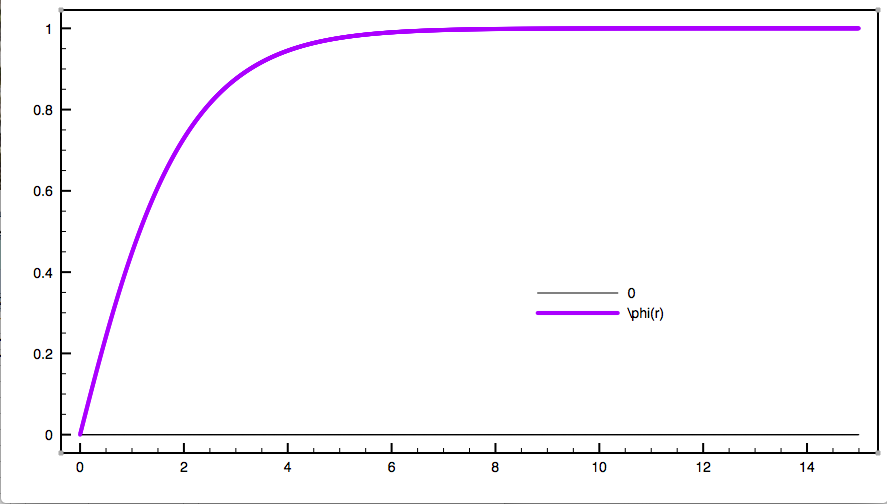
\includegraphics[width=1.\textwidth]{1alilphi.png}
\caption{$\phi(r)$ vs. r for $r\in[eps,15]$ with potential 1 (a) $\rho(r)=\frac{1}{8\pi}e^{-r}$}
\label{1alilphi}
\end{figure}

\begin{figure}[H]
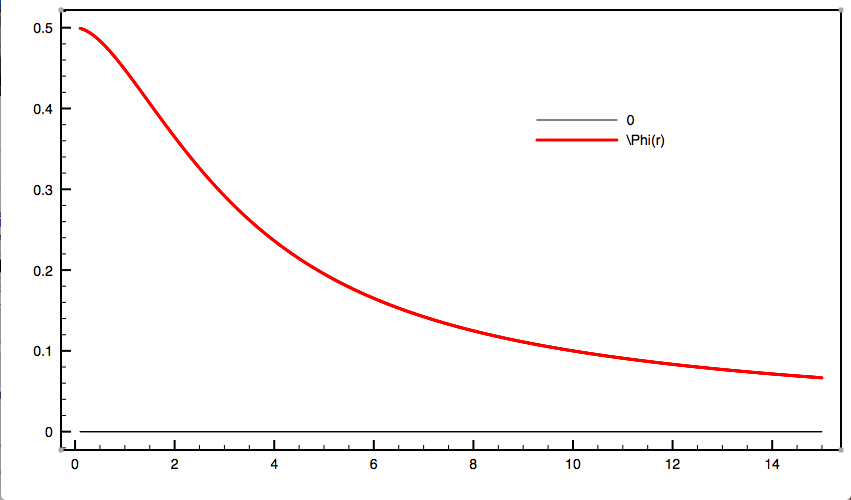
\includegraphics[width=1.\textwidth]{1abigphi.png}
\caption{$\Phi(r)$ vs. r for $r\in(0.1,15]$ with potential 1 (a) $\rho(r)=\frac{1}{8\pi}e^{-r}$}
\label{1abigphi}
\end{figure}

\begin{figure}[H]
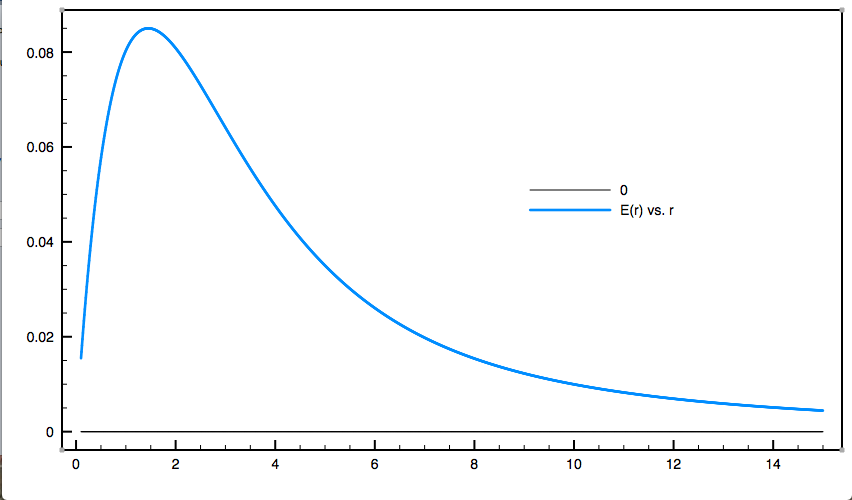
\includegraphics[width=1.\textwidth]{1ae.png}
\caption{$E(r)$ vs. r for $r\in(0.1,15]$ with potential 1 (a) $\rho(r)=\frac{1}{8\pi}e^{-r}$}
\label{1ae}
\end{figure}

\begin{figure}[H]
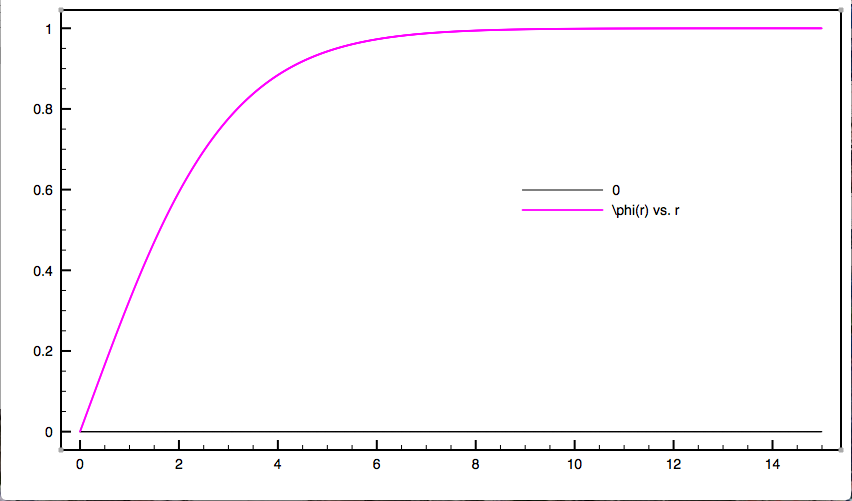
\includegraphics[width=1.\textwidth]{1blilphi.png}
\caption{$\phi(r)$ vs. r for $r\in[eps,15]$ with potential 1 (b) $\rho(r)=\frac{1}{24\pi}re^{-r}$}
\label{1blilphi}
\end{figure}

\begin{figure}[H]
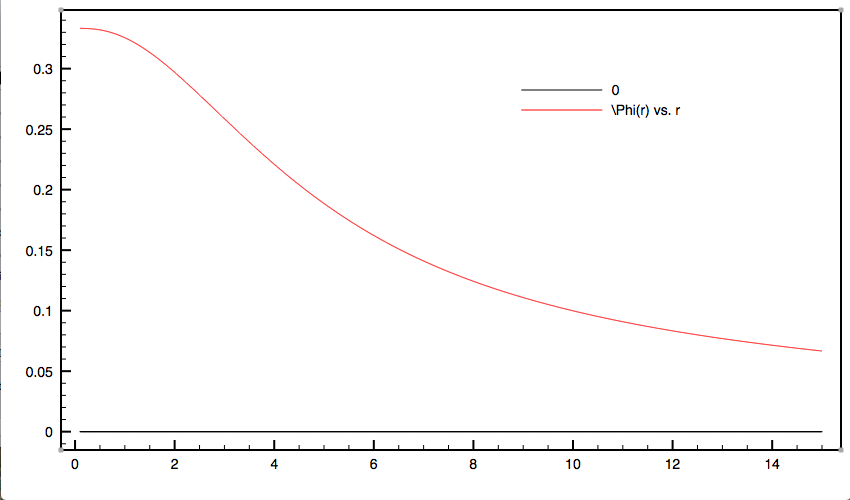
\includegraphics[width=1.\textwidth]{1bbigphi.png}
\caption{$\Phi(r)$ vs. r for $r\in(0.1,15]$ with potential 1 (b) $\rho(r)=\frac{1}{24\pi}re^{-r}$}
\label{1bbigphi}
\end{figure}

\begin{figure}[H]
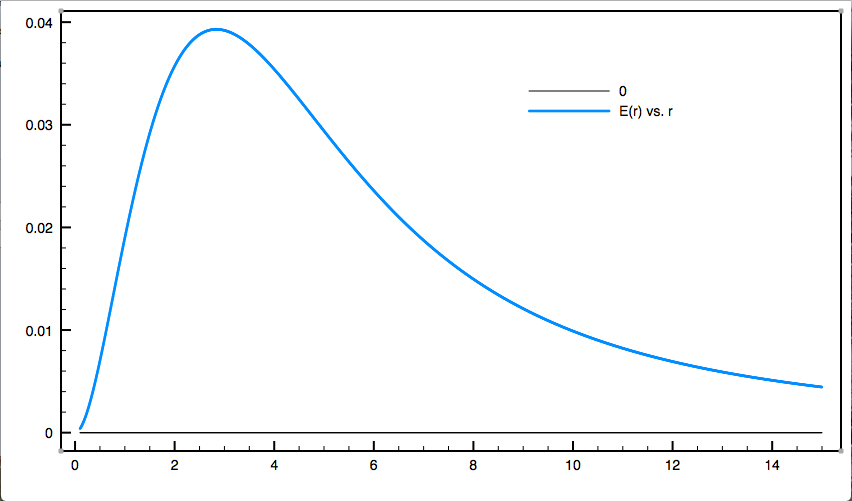
\includegraphics[width=1.\textwidth]{1be.png}
\caption{$E(r)$ vs. r for $r\in(0.1,15]$ with potential 1 (b) $\rho(r)=\frac{1}{24\pi}re^{-r}$}
\label{1be}
\end{figure}

\begin{figure}[H]
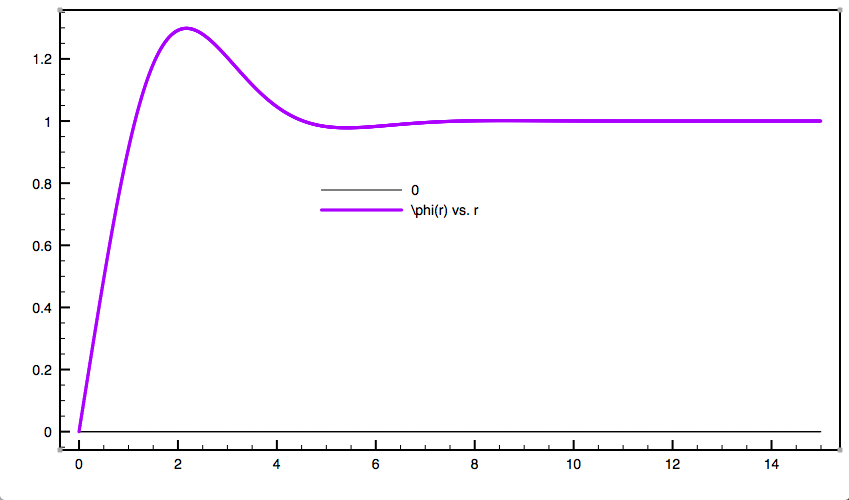
\includegraphics[width=1.\textwidth]{1clilphi.png}
\caption{$\phi(r)$ vs. r for $r\in[eps,15]$ with potential 1 (c) $\rho(r)=\frac{1}{2\pi}\sin(r)e^{-r}$}
\label{1clilphi}
\end{figure}

\begin{figure}[H]
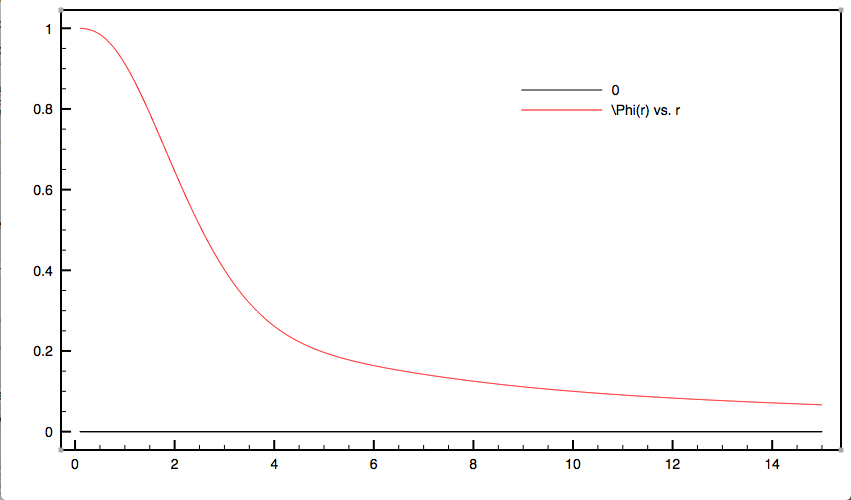
\includegraphics[width=1.\textwidth]{1cbigphi.png}
\caption{$\Phi(r)$ vs. r for $r\in(0.1,15]$ with potential 1 (c) $\rho(r)=\frac{1}{2\pi}\sin(r)e^{-r}$}
\label{1cbigphi}
\end{figure}

\begin{figure}[H]
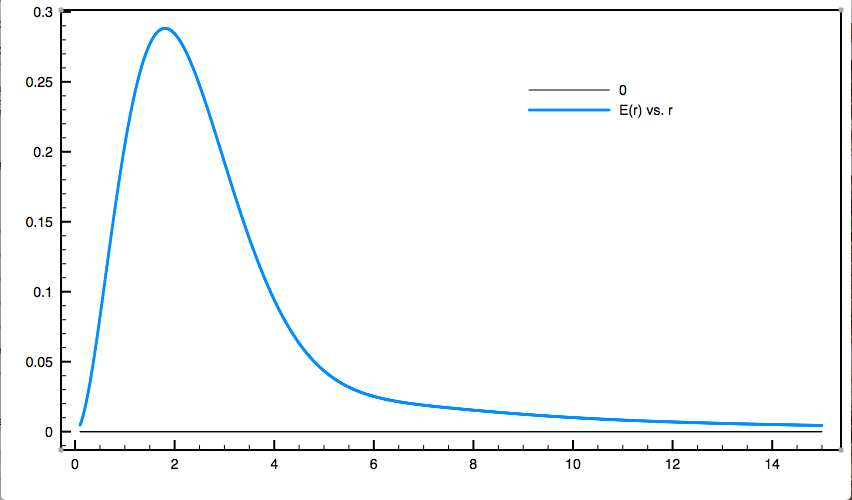
\includegraphics[width=1.\textwidth]{1ce.png}
\caption{$E(r)$ vs. r for $r\in(0.1,15]$ with potential 1 (c) $\rho(r)=\frac{1}{2\pi}\sin(r)e^{-r}$}
\label{1ce}
\end{figure}

\begin{figure}[H]
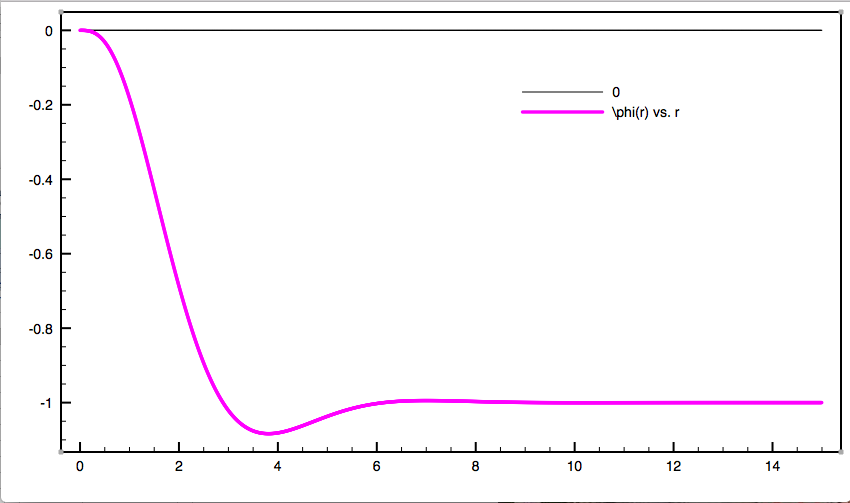
\includegraphics[width=1.\textwidth]{1dlilphi.png}
\caption{$\phi(r)$ vs. r for $r\in[eps,15]$ with potential 1 (d) $\rho(r)=\frac{1}{2\pi}\cos(r)e^{-r}$}
\label{1dlilphi}
\end{figure}

\begin{figure}[H]
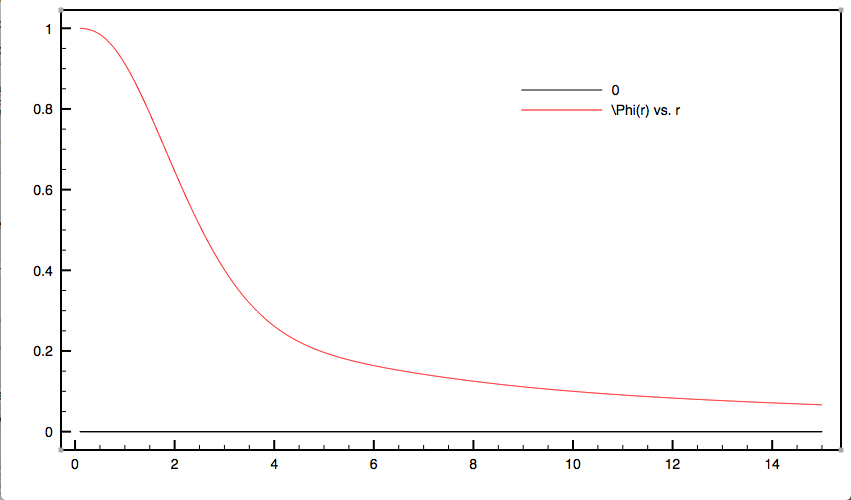
\includegraphics[width=1.\textwidth]{1cbigphi.png}
\caption{$\Phi(r)$ vs. r for $r\in(0.1,15]$ with potential 1 (d) $\rho(r)=\frac{1}{2\pi}\cos(r)e^{-r}$}
\label{1cbigphi}
\end{figure}

\begin{figure}[H]
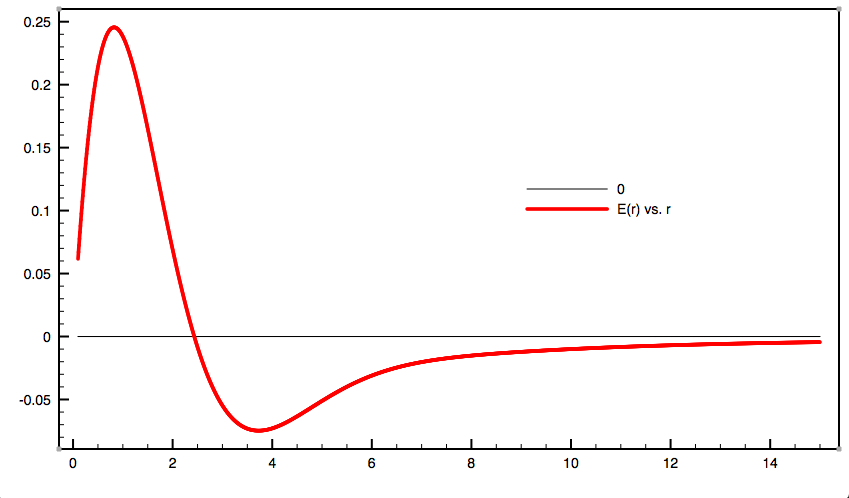
\includegraphics[width=1.\textwidth]{1de.png}
\caption{$E(r)$ vs. r for $r\in(0.1,15]$ with potential 1 (d) $\rho(r)=\frac{1}{2\pi}\cos(r)e^{-r}$}
\label{1blilphi}
\end{figure}

\section{Problem 2}

In Problem 2, we plot the one-dimensional scattering potential corresponding to the data collected below in Listing \ref{scat2} on reflection coefficients $R$ with respect to scattering Energy $E$ (using $m=1$, $\hbar=1$).

\begin{lstlisting}[frame=single,caption={{\tt scat.data}},label=scat2]

1.8   1.00000000
1.9   1.00000000
2.0   0.99999302
2.1   0.95872355
2.2   0.92885044
2.3   0.89392252
2.4   0.85193267
2.5   0.80208166
2.6   0.74443983
2.7   0.67997236
2.8   0.61050692
2.9   0.53853398
3.0   0.46684584
3.1   0.39810686
3.2   0.33448250
3.3   0.27742385
3.4   0.22763279
3.5   0.18516763
3.6   0.14961994
3.7   0.12029981
3.8   0.09639088
3.9   0.07706106
4.0   0.06153060

\end{lstlisting}

The Makefile in Listing \ref{makefile2} provides the instructions for the terminal on how to compile the code.  The {\tt *.f90} files have to be linked together as {\tt *.o} files in the right order, since some of them use subroutines or modules contained in the other ones.  This order is entered from left to right in {\tt objs1}.  Once the object files are linked, they are turned into an executable {\tt scat} such that the code can be run by typing {\tt ./scat} into the terminal in the directory {\tt $\sim$/src}.  The {\tt gfortran} compiler, some flags for optimization, and the library {\tt -framework Accelerate} which contains the linear algebra package {\tt LAPACK} are used here.  The excess files can be cleaned by typing {\tt make clean} into the terminal.

\begin{lstlisting}[frame=single,caption={{\tt Makefile}},label=makefile2]

objs1 = numtype.o setupsch03sc.o rk4step.o downhill-p.o sch03sc.o scatpot.o

prog1 = scat

f90 = gfortran

f90flags = -O3 -funroll-loops -ftree-vectorize -fexternal-blas

libs = -framework Accelerate

ldflags = $(libs)

all: $(prog1)

$(prog1): $(objs1)
	$(f90) $(ldflags) -o $@ $(objs1)

clean: 
	rm -f $(prog1) *.{o,mod} fort.*

.suffixes: $(suffixes) .f90

%.o: %.f90
	$(f90) $(f90flags) -c $<

\end{lstlisting}

The file {\tt numtype.f90} in Listing \ref{numtype2} contains the module {\tt numtype}, which we use to define the precision {\tt dp} of our floating point data types.  We also define the constant {\tt pi}$\equiv\pi$, the complex number {\tt iic}$\equiv i$, and a parameter for very small floating point real data types {\tt tiny}.

\begin{lstlisting}[frame=single,caption={{\tt numtype.f90}},label=numtype2]

module numtype

    save
    integer, parameter :: dp = selected_real_kind(15,307)
    ! integer, parameter :: qp = selected_real_kind(33,4931)
    real(dp), parameter :: pi = 4*atan(1._dp)
    ! defining a complex number
    complex(dp), parameter :: iic = (0._dp,1._dp)
    real(dp), parameter :: tiny = 1.e-30_dp

end module numtype

\end{lstlisting}

The file {\tt setupsch03sc.f90} can be found below in listing \ref{setupsch03sc2}.  It contains the module {\tt setupsch03sc} which contains the number of equations for the Runge-Kutta method subroutine {\tt rk4step}, the values for $m\equiv$ {\tt m}, $\hbar\equiv$ {\tt hbar}, and $\hbar^2\equiv$ {\tt hbar2} stated earlier.  Then it contains the maximum $x$ value used in the subroutine {\tt rk4step}, {\tt xmax}, and the step size, {\tt dstep}.  

\begin{lstlisting}[frame=single,caption={{\tt sch03sc.f90}},label=setupsch03sc2]

module setupsch03sc

    use numtype
	implicit none

	integer, parameter :: n_eq = 2
	real(dp), parameter:: hbar = 1._dp, & 
	hbar2 = hbar**2, mass = 1._dp
    real(dp) :: xmax, dstep

end module setupsch03sc

\end{lstlisting}

The file {\tt rk4step.f90} found in Listing \ref{rk4step2} contains the subroutine {\tt rk4step} which uses the Runge-Kutta method for solving second order differential equations.  We use it to solve for our wavefunction $\psi(x)$ according to the Schrodinger equation, $\frac{d^2\psi(x)}{dx^2}=-\frac{2m}{\hbar^2}(E-V_0)\psi(x)$. 

\begin{lstlisting}[frame=single,caption={{\tt rk4step.f90}},label=rk4step2]

subroutine rk4step(x,h,y, energy, v0, x0)  ! 4-th order Runge-Kutta step
	
	use setupsch03sc, only : dp, n_eq
	implicit none
	real(dp), intent(inout) :: x
	real(dp), intent(in) :: h
	complex(dp), dimension(n_eq), intent(inout) :: y 
	complex(dp), dimension(n_eq) :: k1, k2, k3, k4, dy

	real(dp), intent(in) :: energy, x0, v0
	
	k1 = kv (x, h, y)
	k2 = kv (x+h/2, h, y+k1/2)
	k3 = kv (x+h/2,	h, y+k2/2)
	k4 = kv (x+h, h, y+k3)	

	dy = (k1 + 2*k2 + 2*k3 + k4)/6		! increment
	
	x = x + h                     		! update
	y = y + dy

    contains
    
        function kv (x, dx, y) result(k)  ! derivative

	        use setupsch03sc
	        implicit none
	        real(dp), intent(in) :: x, dx
	        complex(dp), dimension(n_eq), intent(in) :: y
	        complex(dp), dimension(n_eq) :: f, k
			
			f(1) = y(2) 
			
			f(2) = - 2 * mass / hbar2 * ( energy - &
				& potential(x) ) * y(1)
		
			k = dx * f 
	
		end function kv
		
		function potential(x)

			use numtype
			implicit none 
			real(dp) :: x, potential 

			potential = v0 / 2._dp * &
				& ( 1 + tanh(x / x0) )

		end function potential
	
end subroutine rk4step

\end{lstlisting}

The file {\tt downhill-p.f90} can be found below in listing \ref{downhill-p2}.  It contains the subroutine {\tt downhill} which uses the Nelder-Mead method to find the minimum of a function.  

\begin{lstlisting}[frame=single,caption={{\tt downhill-p.f90}},label=downhill-p2]

subroutine downhill(n,func,xstart,fstart,stepi,epsf,itmin,iter)
!
!   n           dimension of the problem
!   func        function
!   xstart      starting values
!   fstart      conrespoding function value
!   stepi       relative stepsize for initial simplex
!   epsf        epsilon for termination
!   itmin       termination is tested if itmin < it
!   iter        maximum number of iterations
!

    use NumType
    implicit none
    integer :: n, iter, itmin
    real(dp), external :: func
    real(dp) :: xstart(1:n), fstart, stepi, epsf
    real(dp), parameter :: alph=1._dp, gamm=2._dp, &
                            rho=0.5_dp, sig=0.5_dp
    real(dp) :: xi(1:n,1:n+1), x(1:n,1:n+1), &
        fi(1:n+1), f(1:n+1),  &
        x0(1:n), xr(1:n), xe(1:n), xc(1:n), &
        fxr, fxe, fxc, deltaf
    integer :: i, ii, it
    
    xi(1:n,1) = xstart(1:n);    fi(1) = fstart
    do i = 2, n+1
        xi(1:n,i)=xi(1:n,1)
        xi(i-1,i)=xi(i-1,i)*(1+stepi)
        fi(i)=func(xi(1:n,i))
    end do
       
    do it = 1, iter 
        
        do i = 1, n+1                           ! ordering
            ii = minloc(fi(1:n+1),dim=1)
            x(1:n,i) = xi(1:n,ii);  f(i) = fi(ii)
            fi(ii) = huge(0._dp)
        end do
        xi(1:n,1:n+1) = x(1:n,1:n+1)
        fi(1:n+1) = f(1:n+1)
                
        x0(1:n) = sum(x(1:n,1:n),dim=2)/n   ! central
        
        if ( itmin < it ) then              ! condition for exit
            deltaf = (f(n)-f(1))
            !write(777,*) it,deltaf
            if(deltaf < epsf ) exit
        end if
                
        xr(1:n) = x0(1:n)+alph*(x0(1:n)-x(1:n,n+1))
        fxr = func(xr)
        if( fxr < f(n) .and. &              ! reflection
                f(1) <= fxr ) then 
            xi(1:n,n+1) = xr(1:n);  fi(n+1) = fxr
            cycle
        
        else if ( fxr < f(1) ) then         ! expansion
            xe(1:n) = x0(1:n)+gamm*(x0(1:n)-x(1:n,n+1))
            fxe = func(xe)
            if( fxe < fxr ) then
                xi(1:n,n+1) = xe(1:n);  fi(n+1) = fxe
                cycle
            else
                xi(1:n,n+1) = xr(1:n);  fi(n+1) = fxr
                cycle
            end if

        else if ( fxr >= f(n) ) then        ! contraction
            xc(1:n) = x(1:n,n+1)+rho*(x0(1:n)-x(1:n,n+1))
            fxc = func(xc)
            if( fxc <= f(n+1) ) then
                xi(1:n,n+1) = xc(1:n);  fi(n+1) = fxc
                cycle
            else                                 ! reduction
                 do i = 2, n+1
                    xi(1:n,i) = x(1:n,1)+sig*(x(1:n,i)-x(1:n,1))
                    fi(i) = func(xi)
                end do
                cycle
            end if
            
        end if
        
    end do
    
    xstart(1:n)=xi(1:n,1); fstart = fi(1)

end subroutine downhill

\end{lstlisting}

The file {\tt sch03sc.f90} can be found below in Listing \ref{sch03sc}.  It contains the subroutine {\tt sch03sc} which calculates and plots the wavefunction satisfying the Schrodinger equation given the parameters {\tt v0} and {\tt x0} for the potential function $V(x)=\frac{{\tt v0}}{2}(1+\tanh(\frac{x}{{\tt x0}}))$.  It calculates the reflection coefficients for a wavefunction which we can use to fit to our data.  

\begin{lstlisting}[frame=single,caption={{\tt sch03sc.f90}},label=sch03sc]

subroutine sch03sc(energy, rr, v0, x0, pr)

    use setupsch03sc
    implicit none
    real(dp) :: x, tt
    complex(dp) :: psi(n_eq), aa, bb, k1, k2

    real(dp), intent(in) :: energy
    real(dp), intent(out) :: rr 
    real(dp), intent(in) :: v0, x0

    integer, intent(in) :: pr

    xmax = 10._dp ! 20._dp
    dstep = 0.001_dp ! 0.001_dp
    x = xmax
   
    ! must add 0*iic to make zqrt argument complex(8)
    k2 = zsqrt(2._dp * mass / hbar2 * ( energy - potential(x) ) + 0._dp * iic)
    psi(1) = exp(iic * k2 * x)
    psi(2) = iic * k2 * psi(1)

    if (pr > 0) then
        do while (x > - xmax) 
            write(19+2*pr, *) x, realpart( psi(1) ), &
                imagpart( psi(1) )
            write(20+2*pr, *) x, potential(x)
            call rk4step(x, - dstep, psi, energy, v0, x0)
        end do
    end if
  

    x = - xmax 

    k1 = zsqrt(2._dp * mass / hbar2 * &
        & ( energy - potential(x) ) + 0._dp * iic)

    aa = ( psi(1) + psi(2) / (iic * k1) ) / &
        & ( 2._dp * exp(iic * k1 * x) )
    bb = ( psi(1) - psi(2) / (iic * k1) ) / &
        & ( 2._dp * exp( - iic * k1 * x) )
    
    rr = abs(bb / aa)**2
    tt = realpart(k2 / k1) * abs(1 / aa)**2

    ! print *, v0, energy, k2, k1
    ! print *, rr, tt, rr + tt 

    contains 

        function potential(z) result(pot)

            use numtype
            implicit none
            real(dp) :: z, pot
        
            pot = v0 / 2._dp * &
                & ( 1._dp + tanh(z / x0) )
        
        end function potential

end subroutine sch03sc

\end{lstlisting}

The file {\tt scatpot.f90} can be found below in Listing \ref{scatpot2}.  It begins with the module {\tt setupscatplot} which provides parameters for the subroutine {\tt downhill} and the function {\tt chi2}.  Program {\tt scatpot} begins with copying the data from {\tt scat.data} into the variables {\tt xx} $\equiv E$ and {\tt yy} $\equiv R$.  Then it runs the subroutine {\tt downhill} which finds the parameters for the potential $V(x)$, {\tt v0} and {\tt x0}, that minimize the function {\tt chi2}.  The function {\tt chi2} measures how well the given parameters for the potential lead to a reflection coefficient as a function of energy that matches the data.  The output and plots of the potential and wavefunctions can be found in the figures below.  The output shows the subroutine {\tt downhill} searching for parameters that best fit the data.

\begin{lstlisting}[frame=single,caption={{\tt elpot.f90}},label=scatpot2]

module setupscatpot

	use numtype
	implicit none

	integer, parameter :: npmax = 50, npar = 2
	real(dp) :: xx(1:npmax), yy(1:npmax)
	integer :: icall, nsp, iprint, nspmin, nspmax
	
end module setupscatpot

program scatpot

    use setupscatpot
    implicit none
    real(dp), external :: chi2
    integer :: i, stat, itmin, itmax
    real(dp) :: xstart(1:npar), fstart, stepi, epsf

    integer :: pr
    pr = 0

    open(unit=2,file='scat.data')
    i = 1
    do
        read(unit=2,fmt='(f5.1,f11.8)', iostat=stat ) xx(i), yy(i)
        if ( stat /= 0 ) exit
        ! print '(i5,2x,f6.2,f10.3)',i,xx(i),yy(i)
        i = i + 1
    end do
    nsp = i-1
    close(2)
    nspmin = 1
    nspmax = nsp

    ! xstart is defined as (v0, x0)
    !  xstart(1:npar)  = (/ 0.2_dp, -0.1_dp /)
    xstart(1:npar) = (/ 2.7846_dp, 1.4162_dp /)
    icall = 0

    iprint = 7
    fstart = chi2(xstart)

    stepi = 0.05_dp
    epsf = 0.001_dp

    itmin = 20
    itmax = 200

    iprint = 0
    
    call downhill(npar,chi2,xstart,fstart,stepi,epsf,itmin,itmax)
 
    iprint = 17
    fstart = chi2(xstart)

    print *, 'v0, x0, chi2'
    print *, xstart(1:npar), fstart

    ! print wavefunction and potential graphs
    do pr = 1, nspmax, 5
        call sch03sc(xx(pr), yy(pr), xstart(1), xstart(2), pr)
    end do
    
end program scatpot

function chi2(par) result(s2)

    use setupscatpot
    implicit none
    real(dp) :: par(npar), x, v0, x0, s2, fi 
    integer :: i 

    real(dp) :: rr

    icall = icall + 1

    v0 = par(1); x0 = par(2)

    s2 = 0
    do i = nspmin, nspmax
        
        x = xx(i) ! x is defined as E
        call sch03sc(x, rr, v0, x0, 0)
        fi = rr 
        s2 = s2 + (yy(i) - fi)**2 / sqrt(yy(i) + 2._dp)

        if ( iprint /= 0 ) then
            ! plot scat.data R(E) vs. E
            write(unit=iprint, fmt='(3f15.5 )' ) x, 0._dp, yy(i)
            ! plot fit rr vs. x
            write(unit=iprint + 1, fmt='(2f15.5 )' ) x, fi 
        end if
    end do 
    s2 = s2 / abs(nspmax - nspmin)

    print '(i5,2x, 8f12.4 )', icall, par(1:npar), s2

end function chi2

\end{lstlisting}

The output of the executable {\tt scatpot} can be found below in Listing \ref{output2}.

\begin{lstlisting}[frame=single,caption={{\tt elpot.f90}},label=output2]

    1        2.7846      1.4162      0.0094
    2        2.9238      1.4162      0.0174
    3        2.7846      1.4870      0.0094
    4        2.6454      1.4870      0.0120
    5        2.8542      1.4339      0.0119
    6        2.7150      1.4693      0.0113
    7        2.8194      1.4428      0.0123
    8        2.7846      1.4870      0.0094
    9        2.7846      1.4870      0.0094
   10        2.7498      1.4782      0.0099
   11        2.8020      1.4649      0.0127
   12        2.7846      1.4870      0.0094
   13        2.7846      1.4870      0.0094
   14        2.7672      1.4826      0.0094
   15        2.7933      1.4759      0.0099
   16        2.7846      1.4870      0.0094
   17        2.7846      1.4870      0.0094
   18        2.7759      1.4848      0.0093
   19        2.7672      1.4870      0.0094
   20        2.7759      1.4936      0.0093
   21        2.7672      1.4914      0.0094
   22        2.7802      1.4881      0.0093
   23        2.7715      1.4903      0.0093
   24        2.7781      1.4887      0.0093
   25        2.7781      1.4798      0.0093
   26        2.7792      1.4729      0.0093
   27        2.7802      1.4837      0.0093
   28        2.7770      1.4845      0.0093
   29        2.7770      1.4757      0.0093
   30        2.7764      1.4692      0.0093
   31        2.7759      1.4804      0.0093
   32        2.7775      1.4800      0.0093
   33        2.7775      1.4711      0.0093
   34        2.7778      1.4644      0.0093
   35        2.7781      1.4754      0.0093
   36        2.7773      1.4756      0.0093
   37        2.7778      1.4755      0.0093
   38        2.7774      1.4756      0.0093
   39        2.7774      1.4667      0.0093
   40        2.7773      1.4601      0.0093
   41        2.7773      1.4712      0.0093
   42        2.7775      1.4711      0.0093
   43        2.7773      1.4712      0.0093
   44        2.7774      1.4711      0.0093
   45        2.7774      1.4623      0.0093
   46        2.7774      1.4556      0.0093
   47        2.7775      1.4667      0.0093
   48        2.7774      1.4667      0.0093
   49        2.7774      1.4623      0.0093
 v0, x0, chi2
   2.7774277514648444        1.4622800915527350        9.2990062482914571E-003
   
\end{lstlisting}

Fig. \ref{refitguess} below shows how well the subroutine {\tt downhill} did at finding parameters to fit the given data.  This looks similar to Fig. \ref{refitdown} because the initial guess I used was already the first result of the {\tt downhill} subroutine, which I thought could be improved upon to no avail.  The following three figures show the plot of the potential barrier that fits the data and three wavefunctions for random incoming energies.

\begin{figure}[H]
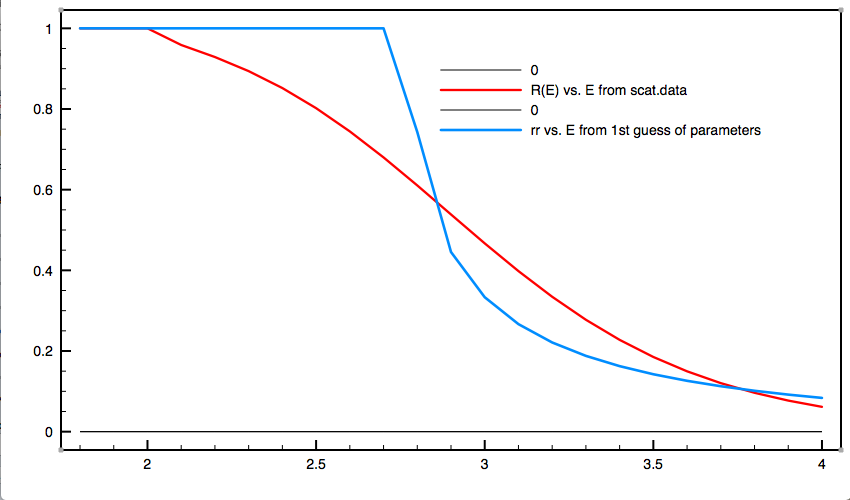
\includegraphics[width=1.\textwidth]{refitguess.png}
\caption{Fit vs. data for initial guess of parameters}
\label{refitguess}
\end{figure}

\begin{figure}[H]
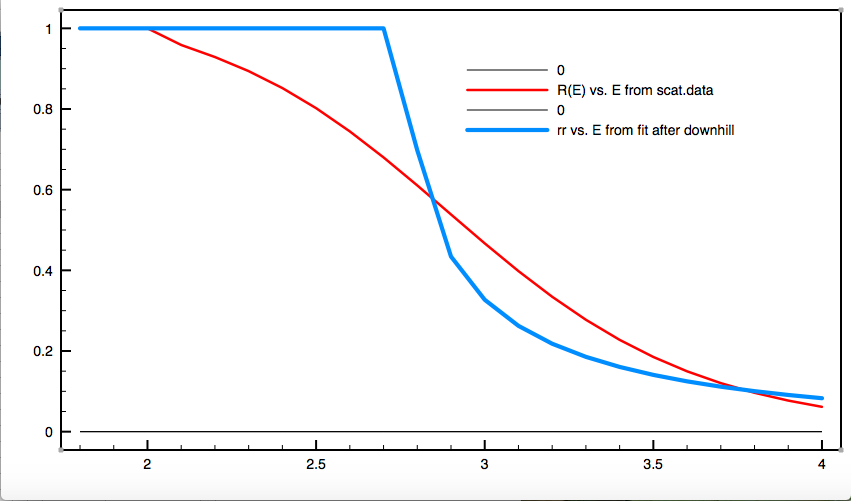
\includegraphics[width=1.\textwidth]{refitdown.png}
\caption{Fit vs. data after parameters were found with {\tt downhill} subroutine}
\label{refitdown}
\end{figure}

\begin{figure}[H]
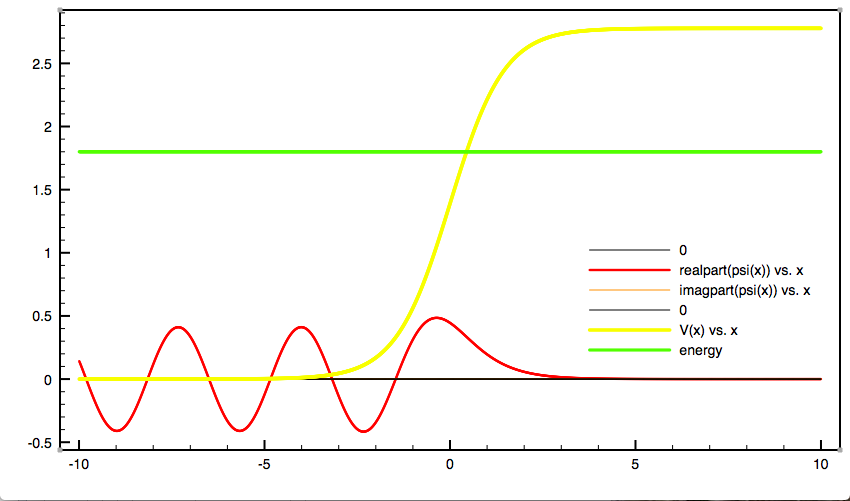
\includegraphics[width=1.\textwidth]{1stwaveplot.png}
\caption{Potential V(x) with parameters fitted by subroutine {\tt downhill} with a wavefunction for a given energy}
\label{1stwaveplot}
\end{figure}

\begin{figure}[H]
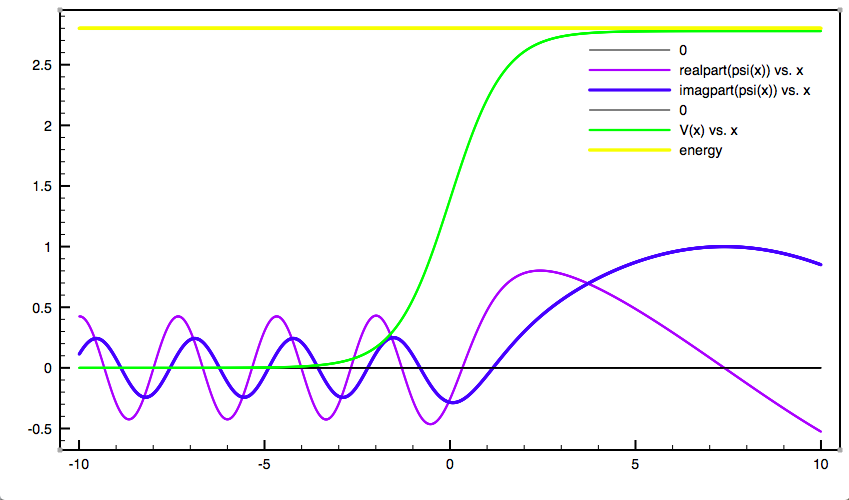
\includegraphics[width=1.\textwidth]{2ndwaveplot.png}
\caption{Potential V(x) with parameters fitted by subroutine {\tt downhill} with a wavefunction for a given energy}
\label{2ndwaveplot}
\end{figure}

\begin{figure}[H]
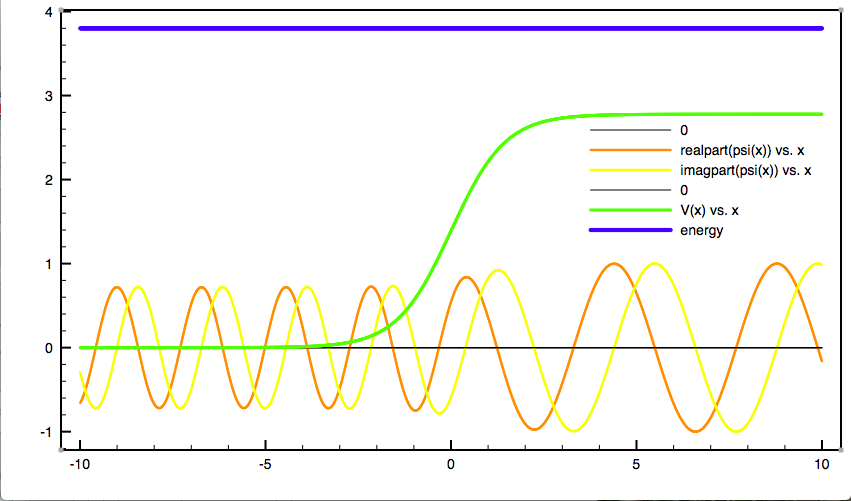
\includegraphics[width=1.\textwidth]{3rdwaveplot.png}
\caption{Potential V(x) with parameters fitted by subroutine {\tt downhill} with a wavefunction for a given energy}
\label{3rdwaveplot}
\end{figure}

\section{Summary and conclusions}

In this final we were reminded of the incredible power computers wield in physics research.  The functions in problem 1 would prove difficult to solve analytically, but take less than one second to be solved computationally.  This power extends far into the world of functions with no analytical solutions but physical applications.  The limits of simulating systems with nonlinear charge distributions have been pushed back considerably by advances in modern computational physics.  

We found the results of Problem 2 to be surprising.  Only that reflection data was necessary to construct an entire potential function responsible for creating this data.  This again urges the incredible power computational physics holds, that physical systems can be reconstructed computationally from experimental data in under a second, when this process would have been incredibly inefficient for a grad student to do by hand in the age before widespread computer usage in physics research.

\begin{thebibliography}{}

\bibitem{poisson} Wikipedia contributors. (2020, April 30). Poisson's equation. {\it In Wikipedia, The Free Encyclopedia}. Retrieved 05:45, May 16, 2020, from \url{https://en.wikipedia.org/w/index.php?title=Poisson%27s_equation&oldid=953991645}

\bibitem{reflection} Wikipedia contributors. (2019, December 5). Transmission coefficient. {\it In Wikipedia, The Free Encyclopedia}. Retrieved 05:45, May 16, 2020, from \url{https://en.wikipedia.org/w/index.php?title=Transmission_coefficient&oldid=929327615}
 
\end{thebibliography}

\end{document}
